
%%%%%%%%%%%%%%%%%% PREAMBULE %%%%%%%%%%%%%%%%%%

\documentclass[aspectratio=169,utf8]{beamer}
%\documentclass[aspectratio=169,handout]{beamer}

\usetheme{Boadilla}
%\usecolortheme{seahorse}
\usecolortheme[RGB={245,66,24}]{structure}
\useoutertheme{infolines}

% packages
\usepackage{amsfonts,amsmath,amssymb,amsthm}
\usepackage[utf8]{inputenc}
\usepackage[T1]{fontenc}
\usepackage{lmodern}

\usepackage[francais]{babel}
\usepackage{fancybox}
\usepackage{graphicx}

\usepackage{float}
\usepackage{xfrac}

%\usepackage[usenames, x11names]{xcolor}
\usepackage{tikz}
\usepackage{pgfplots}
\usepackage{datetime}



%-----  Package unités -----
\usepackage{siunitx}
\sisetup{locale = FR,detect-all,per-mode = symbol}

%\usepackage{mathptmx}
%\usepackage{fouriernc}
%\usepackage{newcent}
%\usepackage[mathcal,mathbf]{euler}

%\usepackage{palatino}
%\usepackage{newcent}
% \usepackage[mathcal,mathbf]{euler}



% \usepackage{hyperref}
% \hypersetup{colorlinks=true, linkcolor=blue, urlcolor=blue,
% pdftitle={Exo7 - Exercices de mathématiques}, pdfauthor={Exo7}}


%section
% \usepackage{sectsty}
% \allsectionsfont{\bf}
%\sectionfont{\color{Tomato3}\upshape\selectfont}
%\subsectionfont{\color{Tomato4}\upshape\selectfont}

%----- Ensembles : entiers, reels, complexes -----
\newcommand{\Nn}{\mathbb{N}} \newcommand{\N}{\mathbb{N}}
\newcommand{\Zz}{\mathbb{Z}} \newcommand{\Z}{\mathbb{Z}}
\newcommand{\Qq}{\mathbb{Q}} \newcommand{\Q}{\mathbb{Q}}
\newcommand{\Rr}{\mathbb{R}} \newcommand{\R}{\mathbb{R}}
\newcommand{\Cc}{\mathbb{C}} 
\newcommand{\Kk}{\mathbb{K}} \newcommand{\K}{\mathbb{K}}

%----- Modifications de symboles -----
\renewcommand{\epsilon}{\varepsilon}
\renewcommand{\Re}{\mathop{\text{Re}}\nolimits}
\renewcommand{\Im}{\mathop{\text{Im}}\nolimits}
%\newcommand{\llbracket}{\left[\kern-0.15em\left[}
%\newcommand{\rrbracket}{\right]\kern-0.15em\right]}

\renewcommand{\ge}{\geqslant}
\renewcommand{\geq}{\geqslant}
\renewcommand{\le}{\leqslant}
\renewcommand{\leq}{\leqslant}
\renewcommand{\epsilon}{\varepsilon}

%----- Fonctions usuelles -----
\newcommand{\ch}{\mathop{\text{ch}}\nolimits}
\newcommand{\sh}{\mathop{\text{sh}}\nolimits}
\renewcommand{\tanh}{\mathop{\text{th}}\nolimits}
\newcommand{\cotan}{\mathop{\text{cotan}}\nolimits}
\newcommand{\Arcsin}{\mathop{\text{arcsin}}\nolimits}
\newcommand{\Arccos}{\mathop{\text{arccos}}\nolimits}
\newcommand{\Arctan}{\mathop{\text{arctan}}\nolimits}
\newcommand{\Argsh}{\mathop{\text{argsh}}\nolimits}
\newcommand{\Argch}{\mathop{\text{argch}}\nolimits}
\newcommand{\Argth}{\mathop{\text{argth}}\nolimits}
\newcommand{\pgcd}{\mathop{\text{pgcd}}\nolimits} 


%----- Commandes divers ------
\newcommand{\ii}{\mathrm{i}}
\newcommand{\dd}{\text{d}}
\newcommand{\id}{\mathop{\text{id}}\nolimits}
\newcommand{\Ker}{\mathop{\text{Ker}}\nolimits}
\newcommand{\Card}{\mathop{\text{Card}}\nolimits}
\newcommand{\Vect}{\mathop{\text{Vect}}\nolimits}
\newcommand{\Mat}{\mathop{\text{Mat}}\nolimits}
\newcommand{\rg}{\mathop{\text{rg}}\nolimits}
\newcommand{\tr}{\mathop{\text{tr}}\nolimits}


%----- Structure des exercices ------

\newtheoremstyle{styleexo}% name
{2ex}% Space above
{3ex}% Space below
{}% Body font
{}% Indent amount 1
{\bfseries} % Theorem head font
{}% Punctuation after theorem head
{\newline}% Space after theorem head 2
{}% Theorem head spec (can be left empty, meaning ‘normal’)

%\theoremstyle{styleexo}
\newtheorem{exo}{Exercice}
\newtheorem{ind}{Indications}
\newtheorem{cor}{Correction}


\newcommand{\exercice}[1]{} \newcommand{\finexercice}{}
%\newcommand{\exercice}[1]{{\tiny\texttt{#1}}\vspace{-2ex}} % pour afficher le numero absolu, l'auteur...
\newcommand{\enonce}{\begin{exo}} \newcommand{\finenonce}{\end{exo}}
\newcommand{\indication}{\begin{ind}} \newcommand{\finindication}{\end{ind}}
\newcommand{\correction}{\begin{cor}} \newcommand{\fincorrection}{\end{cor}}

\newcommand{\noindication}{\stepcounter{ind}}
\newcommand{\nocorrection}{\stepcounter{cor}}

\newcommand{\fiche}[1]{} \newcommand{\finfiche}{}
\newcommand{\titre}[1]{\centerline{\large \bf #1}}
\newcommand{\addcommand}[1]{}
\newcommand{\video}[1]{}

% Marge
\newcommand{\mymargin}[1]{\marginpar{{\small #1}}}

\def\noqed{\renewcommand{\qedsymbol}{}}


%----- Presentation ------
\setlength{\parindent}{0cm}

%\newcommand{\ExoSept}{\href{http://exo7.emath.fr}{\textbf{\textsf{Exo7}}}}

\definecolor{myred}{rgb}{0.93,0.26,0}
\definecolor{myorange}{rgb}{0.97,0.58,0}
\definecolor{myyellow}{rgb}{1,0.86,0}

\newcommand{\LogoExoSept}[1]{  % input : echelle
{\usefont{U}{cmss}{bx}{n}
\begin{tikzpicture}[scale=0.1*#1,transform shape]
  \fill[color=myorange] (0,0)--(4,0)--(4,-4)--(0,-4)--cycle;
  \fill[color=myred] (0,0)--(0,3)--(-3,3)--(-3,0)--cycle;
  \fill[color=myyellow] (4,0)--(7,4)--(3,7)--(0,3)--cycle;
  \node[scale=5] at (3.5,3.5) {Exo7};
\end{tikzpicture}}
}


\newcommand{\debutmontitre}{
  \author{} \date{} 
  \thispagestyle{empty}
  \hspace*{-10ex}
  \begin{minipage}{\textwidth}
    \titlepage  
  \vspace*{-2.5cm}
  \begin{center}
    \LogoExoSept{2.5}
  \end{center}
  \end{minipage}

  \vspace*{-0cm}
  
  % Astuce pour que le background ne soit pas discrétisé lors de la conversion pdf -> png
\begin{tikzpicture}
        \fill[opacity=0,green!60!black] (0,0)--++(0,0)--++(0,0)--++(0,0)--cycle; 
\end{tikzpicture}

% toc S'affiche trop tot :
% \tableofcontents[hideallsubsections, pausesections]
}

\newcommand{\finmontitre}{
  \end{frame}
  \setcounter{framenumber}{0}
} % ne marche pas pour une raison obscure

%----- Commandes supplementaires ------

% \usepackage[landscape]{geometry}
% \geometry{top=1cm, bottom=3cm, left=2cm, right=10cm, marginparsep=1cm
% }
% \usepackage[a4paper]{geometry}
% \geometry{top=2cm, bottom=2cm, left=2cm, right=2cm, marginparsep=1cm
% }

%\usepackage{standalone}


% New command Arnaud -- november 2011
\setbeamersize{text margin left=24ex}
% si vous modifier cette valeur il faut aussi
% modifier le decalage du titre pour compenser
% (ex : ici =+10ex, titre =-5ex

\theoremstyle{definition}
%\newtheorem{proposition}{Proposition}
%\newtheorem{exemple}{Exemple}
%\newtheorem{theoreme}{Théorème}
%\newtheorem{lemme}{Lemme}
%\newtheorem{corollaire}{Corollaire}
%\newtheorem*{remarque*}{Remarque}
%\newtheorem*{miniexercice}{Mini-exercices}
%\newtheorem{definition}{Définition}

% Commande tikz
\usetikzlibrary{calc}
\usetikzlibrary{patterns,arrows}
\usetikzlibrary{matrix}
\usetikzlibrary{fadings} 

%definition d'un terme
\newcommand{\defi}[1]{{\color{myorange}\textbf{\emph{#1}}}}
\newcommand{\evidence}[1]{{\color{blue}\textbf{\emph{#1}}}}
\newcommand{\assertion}[1]{\emph{\og#1\fg}}  % pour chapitre logique
%\renewcommand{\contentsname}{Sommaire}
\renewcommand{\contentsname}{}
\setcounter{tocdepth}{2}



%------ Figures ------

\def\myscale{1} % par défaut 
\newcommand{\myfigure}[2]{  % entrée : echelle, fichier figure
\def\myscale{#1}
\begin{center}
\footnotesize
{#2}
\end{center}}


%------ Encadrement ------

\usepackage{fancybox}


\newcommand{\mybox}[1]{
\setlength{\fboxsep}{7pt}
\begin{center}
\shadowbox{#1}
\end{center}}

\newcommand{\myboxinline}[1]{
\setlength{\fboxsep}{5pt}
\raisebox{-10pt}{
\shadowbox{#1}
}
}

%--------------- Commande beamer---------------
\newcommand{\beameronly}[1]{#1} % permet de mettre des pause dans beamer pas dans poly


\setbeamertemplate{navigation symbols}{}
\setbeamertemplate{footline}  % tiré du fichier beamerouterinfolines.sty
{
  \leavevmode%
  \hbox{%
  \begin{beamercolorbox}[wd=.333333\paperwidth,ht=2.25ex,dp=1ex,center]{author in head/foot}%
    % \usebeamerfont{author in head/foot}\insertshortauthor%~~(\insertshortinstitute)
    \usebeamerfont{section in head/foot}{\bf\insertshorttitle}
  \end{beamercolorbox}%
  \begin{beamercolorbox}[wd=.333333\paperwidth,ht=2.25ex,dp=1ex,center]{title in head/foot}%
    \usebeamerfont{section in head/foot}{\bf\insertsectionhead}
  \end{beamercolorbox}%
  \begin{beamercolorbox}[wd=.333333\paperwidth,ht=2.25ex,dp=1ex,right]{date in head/foot}%
    % \usebeamerfont{date in head/foot}\insertshortdate{}\hspace*{2em}
    \insertframenumber{} / \inserttotalframenumber\hspace*{2ex} 
  \end{beamercolorbox}}%
  \vskip0pt%
}


\definecolor{mygrey}{rgb}{0.5,0.5,0.5}
\setlength{\parindent}{0cm}
%\DeclareTextFontCommand{\helvetica}{\fontfamily{phv}\selectfont}

% background beamer
\definecolor{couleurhaut}{rgb}{0.85,0.9,1}  % creme
\definecolor{couleurmilieu}{rgb}{1,1,1}  % vert pale
\definecolor{couleurbas}{rgb}{0.85,0.9,1}  % blanc
\setbeamertemplate{background canvas}[vertical shading]%
[top=couleurhaut,middle=couleurmilieu,midpoint=0.4,bottom=couleurbas] 
%[top=fondtitre!05,bottom=fondtitre!60]



\makeatletter
\setbeamertemplate{theorem begin}
{%
  \begin{\inserttheoremblockenv}
  {%
    \inserttheoremheadfont
    \inserttheoremname
    \inserttheoremnumber
    \ifx\inserttheoremaddition\@empty\else\ (\inserttheoremaddition)\fi%
    \inserttheorempunctuation
  }%
}
\setbeamertemplate{theorem end}{\end{\inserttheoremblockenv}}

\newenvironment{theoreme}[1][]{%
   \setbeamercolor{block title}{fg=structure,bg=structure!40}
   \setbeamercolor{block body}{fg=black,bg=structure!10}
   \begin{block}{{\bf Th\'eor\`eme }#1}
}{%
   \end{block}%
}


\newenvironment{proposition}[1][]{%
   \setbeamercolor{block title}{fg=structure,bg=structure!40}
   \setbeamercolor{block body}{fg=black,bg=structure!10}
   \begin{block}{{\bf Proposition }#1}
}{%
   \end{block}%
}

\newenvironment{corollaire}[1][]{%
   \setbeamercolor{block title}{fg=structure,bg=structure!40}
   \setbeamercolor{block body}{fg=black,bg=structure!10}
   \begin{block}{{\bf Corollaire }#1}
}{%
   \end{block}%
}

\newenvironment{mydefinition}[1][]{%
   \setbeamercolor{block title}{fg=structure,bg=structure!40}
   \setbeamercolor{block body}{fg=black,bg=structure!10}
   \begin{block}{{\bf Définition} #1}
}{%
   \end{block}%
}

\newenvironment{lemme}[0]{%
   \setbeamercolor{block title}{fg=structure,bg=structure!40}
   \setbeamercolor{block body}{fg=black,bg=structure!10}
   \begin{block}{\bf Lemme}
}{%
   \end{block}%
}

\newenvironment{remarque}[1][]{%
   \setbeamercolor{block title}{fg=black,bg=structure!20}
   \setbeamercolor{block body}{fg=black,bg=structure!5}
   \begin{block}{Remarque #1}
}{%
   \end{block}%
}


\newenvironment{exemple}[1][]{%
   \setbeamercolor{block title}{fg=black,bg=structure!20}
   \setbeamercolor{block body}{fg=black,bg=structure!5}
   \begin{block}{{\bf Exemple }#1}
}{%
   \end{block}%
}


\newenvironment{miniexercice}[0]{%
   \setbeamercolor{block title}{fg=structure,bg=structure!20}
   \setbeamercolor{block body}{fg=black,bg=structure!5}
   \begin{block}{Mini-exercices}
}{%
   \end{block}%
}


\newenvironment{tp}[0]{%
   \setbeamercolor{block title}{fg=structure,bg=structure!40}
   \setbeamercolor{block body}{fg=black,bg=structure!10}
   \begin{block}{\bf Travaux pratiques}
}{%
   \end{block}%
}
\newenvironment{exercicecours}[1][]{%
   \setbeamercolor{block title}{fg=structure,bg=structure!40}
   \setbeamercolor{block body}{fg=black,bg=structure!10}
   \begin{block}{{\bf Exercice }#1}
}{%
   \end{block}%
}
\newenvironment{algo}[1][]{%
   \setbeamercolor{block title}{fg=structure,bg=structure!40}
   \setbeamercolor{block body}{fg=black,bg=structure!10}
   \begin{block}{{\bf Algorithme}\hfill{\color{gray}\texttt{#1}}}
}{%
   \end{block}%
}


\setbeamertemplate{proof begin}{
   \setbeamercolor{block title}{fg=black,bg=structure!20}
   \setbeamercolor{block body}{fg=black,bg=structure!5}
   \begin{block}{{\footnotesize Démonstration}}
   \footnotesize
   \smallskip}
\setbeamertemplate{proof end}{%
   \end{block}}
\setbeamertemplate{qed symbol}{\openbox}


\makeatother
\usecolortheme[RGB={192,41,0}]{structure}

% Commande spécifique à ce chapitre
\newcommand{\Sage}{\texttt{Sage}}

\usepackage{textcomp}

\usepackage{listings}
\lstset{
  upquote=true,
  columns=flexible,
  keepspaces=true,
  basicstyle=\ttfamily,
  commentstyle=\color{gray},
  language=Python,
  showstringspaces=false,
  aboveskip=0em,  
  belowskip=0em,
  escapeinside=||,
  breaklines=true,
  postbreak=\raisebox{0ex}[0ex][0ex]{\qquad\ensuremath{\color{red}\hookrightarrow\space}},
}

\lstset{
  literate={é}{{\'e}}1
           {è}{{\`e}}1
           {à}{{\`a}}1
}

\newcommand{\codeinline}[1]{\lstinline!#1!}


   
%%%%%%%%%%%%%%%%%%%%%%%%%%%%%%%%%%%%%%%%%%%%%%%%%%%%%%%%%%%%%
%%%%%%%%%%%%%%%%%%%%%%%%%%%%%%%%%%%%%%%%%%%%%%%%%%%%%%%%%%%%%


\begin{document}


\title{{\bf Calcul formel}}
\subtitle{Courbes et surfaces (1)}

\begin{frame}
  
  \debutmontitre

  \pause

{\footnotesize
\hfill
\setbeamercovered{transparent=50}
\begin{minipage}{0.6\textwidth}
  \begin{itemize}
    \item<3-> Courbes paramétrées
    \item<4-> Courbes en coordonnées polaires
    \item<5-> Courbes définies par une équation
    \item<6-> Surfaces
  \end{itemize}
\end{minipage}
}

\end{frame}

\setcounter{framenumber}{0}



%%%%%%%%%%%%%%%%%%%%%%%%%%%%%%%%%%%%%%%%%%%%%%%%%%%%%%%%%%%%%%%%
\section{Courbes paramétrées}

\begin{frame}[fragile]

\begin{itemize}
  \item \codeinline{plot(sin(x)*exp(x), (x, -3, 3))}
  \uncover<2->{\item Courbe paramétrée plane $(f(t), g(t))$, $t \in [a,b]$}
  \uncover<3->{\item \codeinline{parametric_plot( (f(t), g(t)), (t, a, b) )}}
\end{itemize}

\begin{center}
 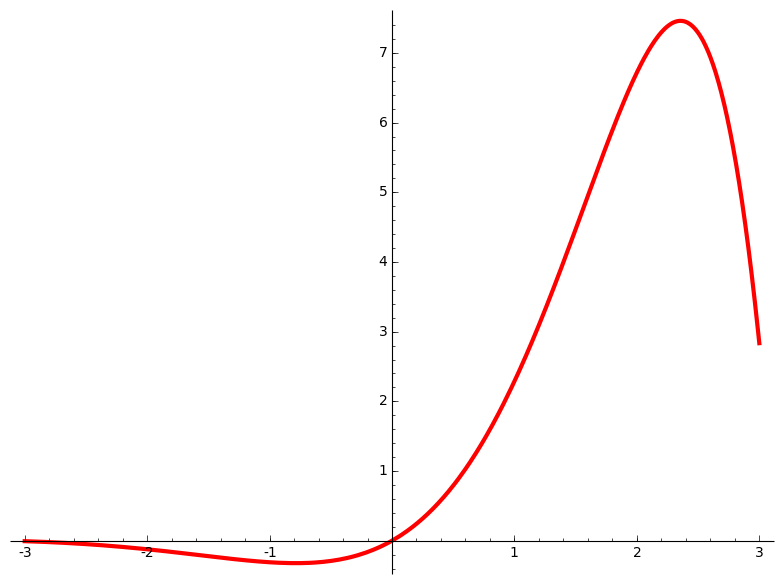
\includegraphics[scale=0.2]{figures/intro_courbes} \qquad
 \uncover<4->{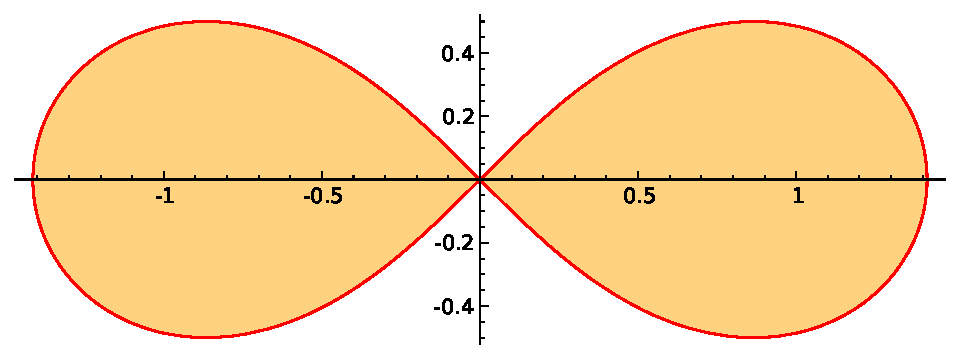
\includegraphics[scale=0.35]{figures/lemniscate_bernoulli}}
\end{center}

\pause\pause\pause
\begin{algo}[lemniscate-bernoulli.sage]
\begin{lstlisting}
var('t')
x = sqrt(2)*cos(t)/(1+sin(t)^2)
y = sqrt(2)*cos(t)*sin(t)/(1+sin(t)^2)
G = parametric_plot((x, y), (t, 0, 2*pi))
G.show()
\end{lstlisting}
\end{algo}


\end{frame}


\begin{frame}
\begin{tp}
\begin{enumerate}
  \item Tracer la spirale de Fermat d'équation
  $$\left\{
\begin{array}{l}
x(t)=\sqrt t \cos t\\[1mm]
y(t)=\sqrt t \sin t
\end{array}
\right. \qquad t \in \Rr_+.$$
  \item Tracer la courbe du papillon
  $$\left\{
\begin{array}{l}
x(t) = \sin(t)\left(\exp(\cos(t))-2\cos(4t)-\sin^5\left(\frac{t}{12}\right)\right)\\[3mm]
y(t) = \cos(t)\left(\exp(\cos(t))-2\cos(4t)-\sin^5\left(\frac{t}{12}\right)\right)
\end{array}
\right. \qquad t \in \Rr.$$
\end{enumerate} 
\end{tp}

\end{frame}


\begin{frame}[fragile]
\begin{center}
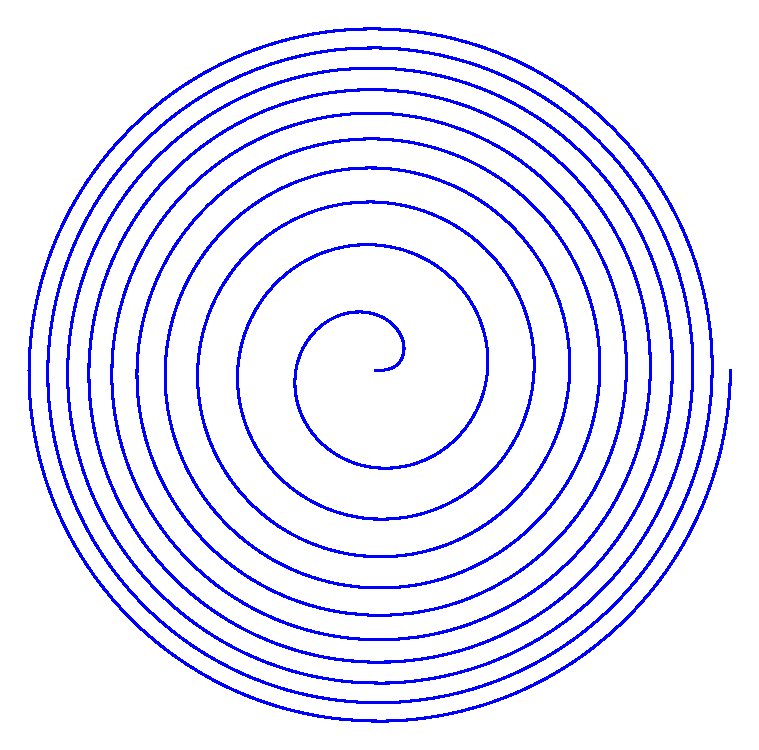
\includegraphics[scale=0.3]{figures/fermat_spiral}\quad
\includegraphics[scale=0.255]{figures/butterfly_curve}  
\end{center}

\pause

Options de tracé à découvrir grâce 
à \codeinline{help(parametric_plot)} 

\pause
\begin{itemize}
  \item Imposer un repère orthonormé : \codeinline{aspect_ratio = 1}
\pause
  \item Nombre de points pour le tracé : \codeinline{plot_points = 500}
\pause    
  \item Ne pas afficher les axes : \codeinline{axes = False}
\pause  
  \item Afficher une grille : \codeinline{gridlines = True}
\pause  
  \item Couleur du trait : \codeinline{color = 'red'}

\end{itemize}
\end{frame}




%%%%%%%%%%%%%%%%%%%%%%%%%%%%%%%%%%%%%%%%%%%%%%%%%%%%%%%%%%%%%%%%
\section{Courbes en coordonnées polaires}

\begin{frame}[fragile]

\begin{itemize}
  \item Courbe en coordonnées polaires $[r(t):t]$, $t \in [a,b]$
  \pause
  \item \codeinline{polar_plot(r(t), (t, a, b))}
  \pause
  \item Folium de Dürer d'équation 
$r(t) = \sin \frac t 2$, $t \in \Rr$
\end{itemize}

\begin{center}
 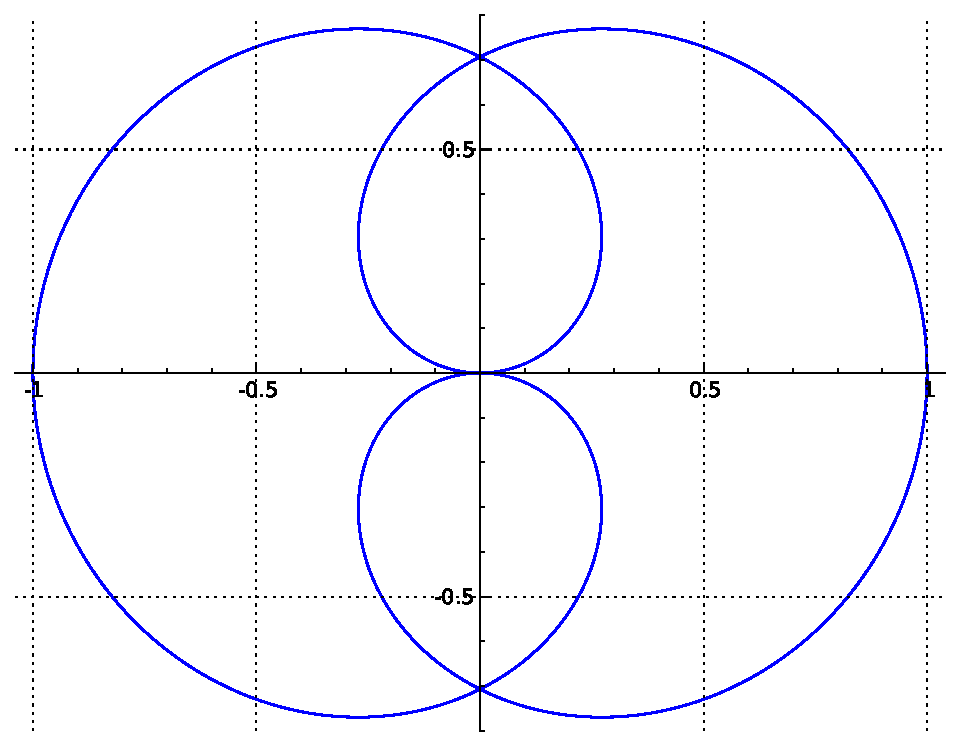
\includegraphics[scale=0.30]{figures/durer_folium} 
\end{center}

  \pause
\begin{algo}[durer-folium.sage]
\begin{lstlisting}
var('t')
G = polar_plot(sin(t/2), (t, 0, 4*pi))
G.show()
\end{lstlisting}
\end{algo}

\end{frame}


\begin{frame}[fragile]


\begin{tp}
\begin{enumerate}
  \item Tracer la courbe du Lituus d'équation polaire 
  $r(t)^2 = \frac{1}{t}$, $t \in \Rr^*$.
  \item Tracer la cochléoïde d'équation polaire 
	  $r(t) = \frac{\sin t}{t}$, $t \in \Rr^*$.
\end{enumerate} 
\end{tp}

\uncover<4->{
Indication : définir deux graphes \codeinline{G1}, 
\codeinline{G2} pour chacun des intervalles de définition. Superposer
les par \codeinline{G = G1+G2}, puis afficher avec 
\codeinline{G.show()}
}

\begin{center}
\begin{minipage}{0.45\textwidth}
\uncover<2->{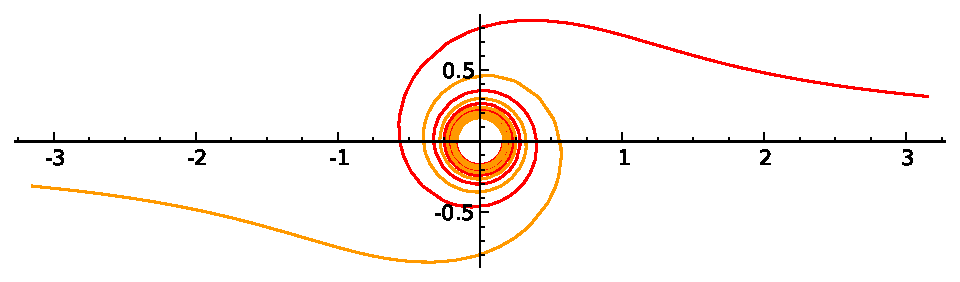
\includegraphics[scale=0.49]{figures/lituus}}
\end{minipage}\ 
\begin{minipage}{0.49\textwidth}
\uncover<3->{\qquad\qquad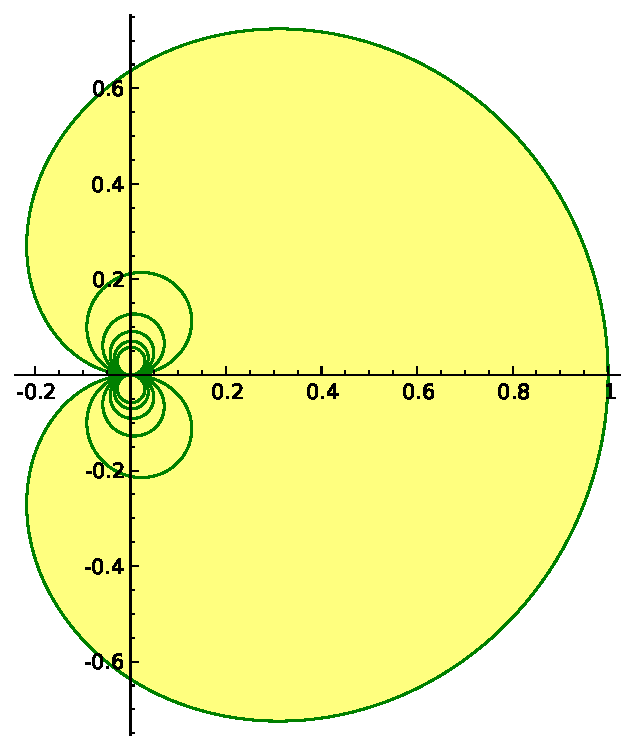
\includegraphics[scale=0.35]{figures/cochleoid} }
\end{minipage}
\end{center}
\end{frame}



%%%%%%%%%%%%%%%%%%%%%%%%%%%%%%%%%%%%%%%%%%%%%%%%%%%%%%%%%%%%%%%%
\section{Courbes définies par une équation}

\begin{frame}[fragile]

\begin{minipage}{0.65\textwidth}
\begin{itemize}
  \item \'Equation implicite du cercle : $x^2+y^2 = 1$
  \pause
  \item \'Equation implicite : $f(x,y)=0$ 
  \pause
  \item Tracer l'ensemble des couples $(x,y)$ dans $[a,b]\times[c,d]$ qui sont solutions de l'équation 
$f(x,y)=0$
\end{itemize}
\end{minipage}
\begin{minipage}{0.29\textwidth}
\begin{center}
  \uncover<5->{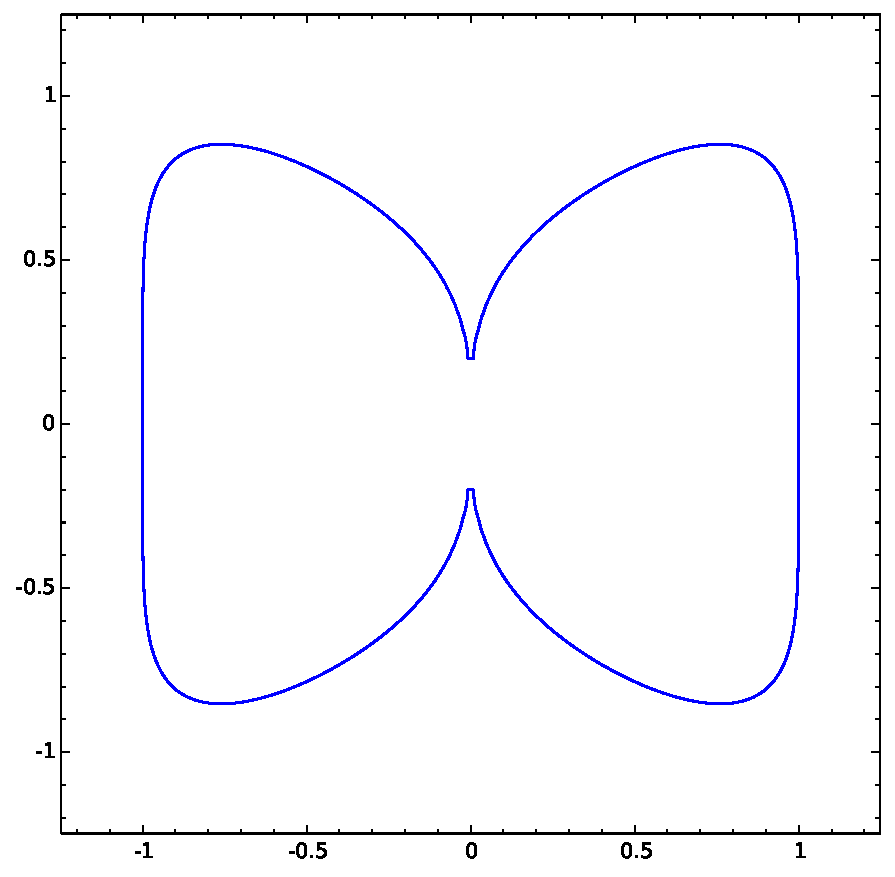
\includegraphics[scale=0.25]{figures/butterfly_curve_algebraic}}
\end{center}
\end{minipage}
\pause
\begin{itemize}
  \item \codeinline{implicit_plot(f(x,y), (x, a, b), (y, c, d))}
\end{itemize}
\pause\pause
\begin{algo}[butterfly-curve-algebraic.sage]
\begin{lstlisting}
f(x,y) = x^6 + y^6 - x^2
G = implicit_plot(f, (x, -1.2, 1.2), (y, -1.2, 1.2))
G.show()
G.save('butterfly_curve_algebraic.png')
\end{lstlisting}
\end{algo}
\end{frame}


\begin{frame}[fragile]
\begin{tp}
\begin{enumerate}
  \item Définir une fonction qui renvoie la courbe définie par
  $$y^2-x^3+x+c = 0$$
  en fonction du paramètre $c\in \Rr$.
  \item \`A l'aide de la commande \codeinline{animate}, 
  réaliser une animation qui affiche l'évolution de la courbe
  pour $c \in[-1,1]$.
\end{enumerate}
\end{tp}


\begin{center}
\uncover<2->{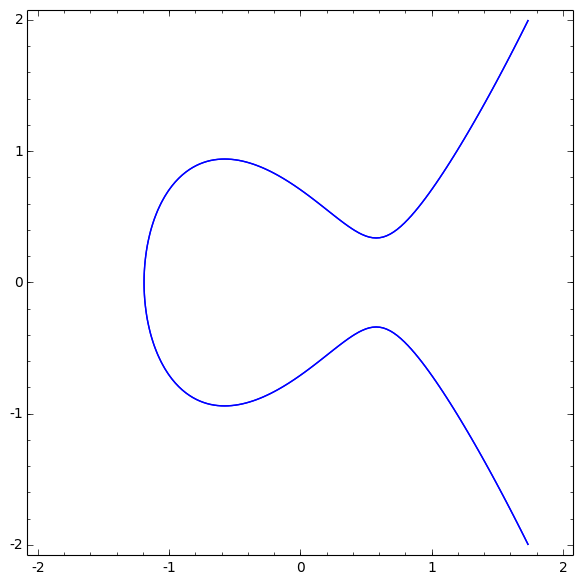
\includegraphics[scale=0.23]{figures/elliptic1}\quad}
\uncover<3->{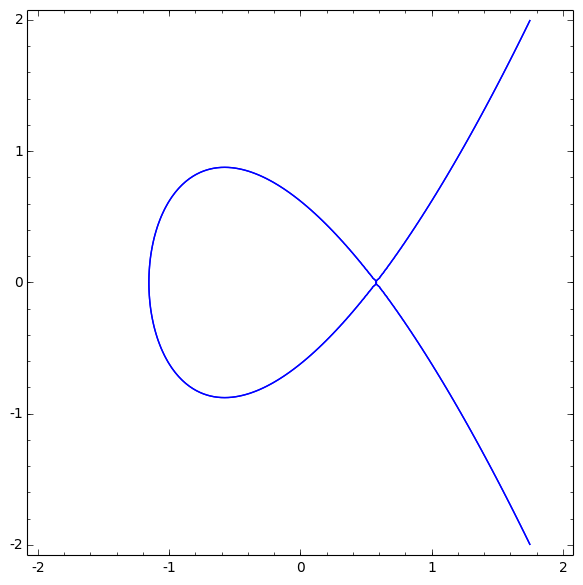
\includegraphics[scale=0.23]{figures/elliptic2}\quad}
\uncover<4->{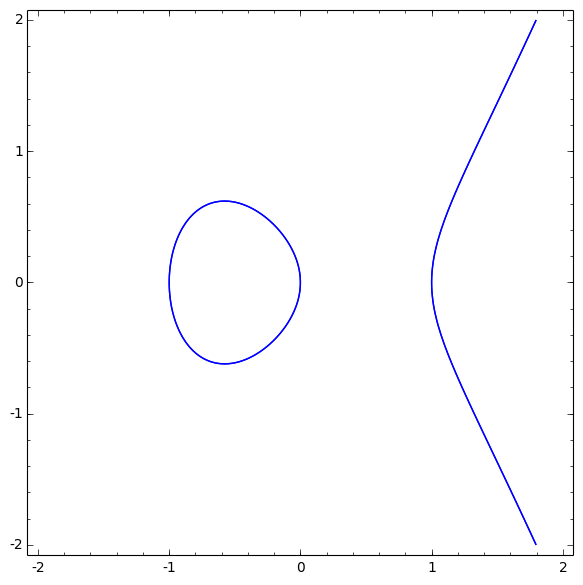
\includegraphics[scale=0.23]{figures/elliptic3}}
\end{center}
\end{frame}




%%%%%%%%%%%%%%%%%%%%%%%%%%%%%%%%%%%%%%%%%%%%%%%%%%%%%%%%%%%%%%%%%
%\section{Courbes de l'espace}
%
%\begin{frame}
%La commande \codeinline{parametric_plot((x, y, z), (t, a, b))}, 
%(ou bien \codeinline{parametric_plot3d()}) analogue à celle de la dimension $2$, 
%trace la courbe paramétrée de 
%l'espace donnée par les points de coordonnées $\big( x(t), y(t), z(t) \big)$ 
%lorsque le paramètre $t$ varie dans l'intervalle $[a,b]$. 
%
%\begin{tp}
%Tracer la courbe d'Archytas d'équation paramétrique :
%$$\left\{
%\begin{array}{l}
%x(t) = \cos^2 t \\[1mm]
%y(t) = \cos t \sin t \\[1mm]
%z(t) = \pm\sqrt{ \cos t(1-\cos t) }
%\end{array}
%\right.\qquad  t \in \big[-\tfrac\pi2,+\tfrac\pi2\big].$$
%\end{tp}
%
%%\insertcode{formel/Algos/archytas_curve.sage}{archytas-curve.sage}
%
%Vous obtiendrez une figure qu'il est possible d'orienter dynamiquement 
%avec la souris. Voici quelques-unes de ces vues.
%
%\begin{center}
% 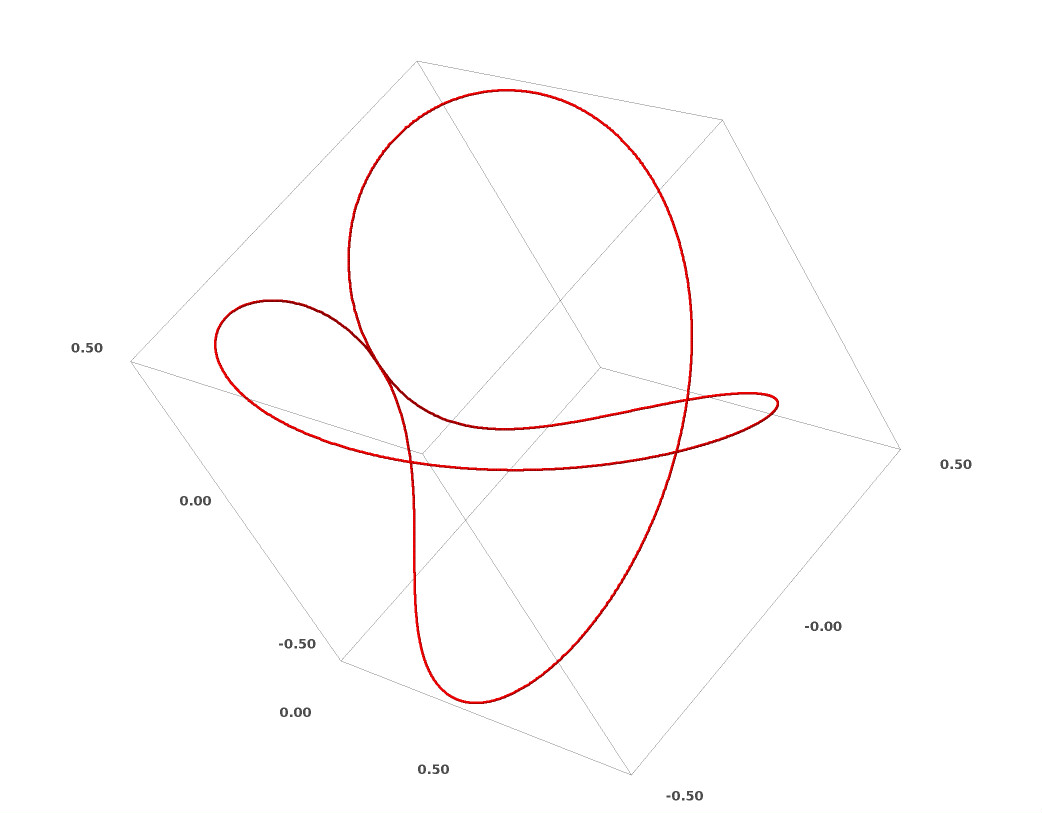
\includegraphics[scale=0.2]{figures/archytas_curve_new1.jpg} 
%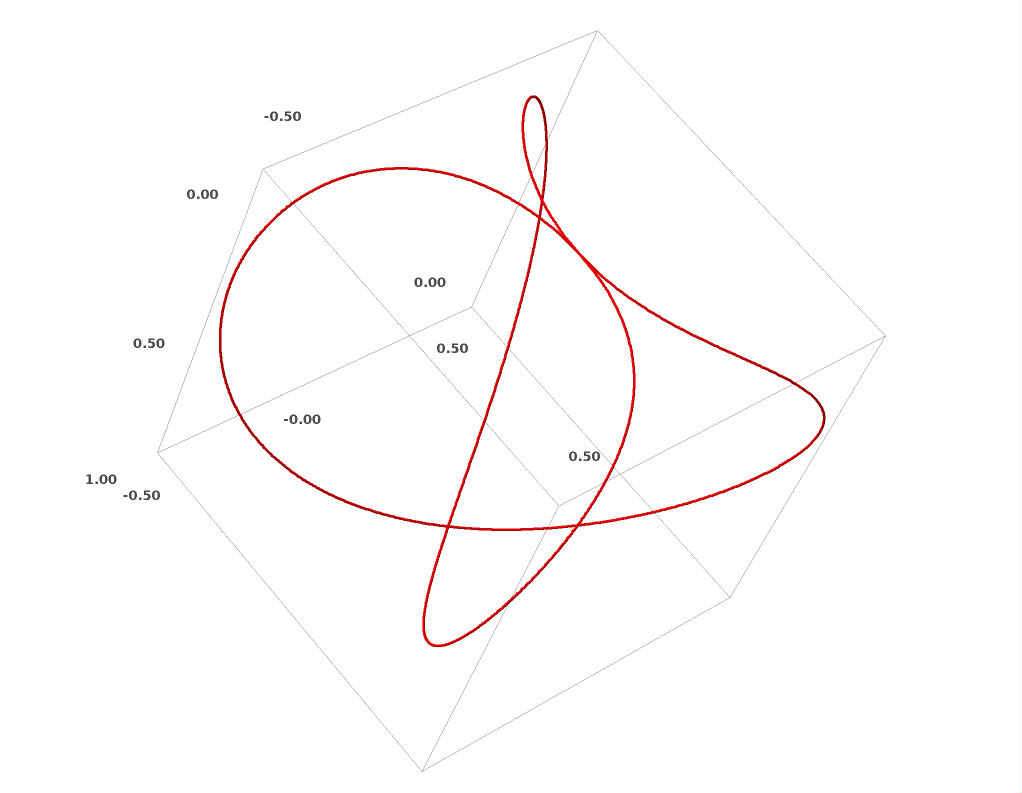
\includegraphics[scale=0.2]{figures/archytas_curve_new2.jpg}  
%\end{center}
%\end{frame}




%%%%%%%%%%%%%%%%%%%%%%%%%%%%%%%%%%%%%%%%%%%%%%%%%%%%%%%%%%%%%%%%
\section{Surfaces}

\begin{frame}


\begin{tp}
\begin{enumerate}
  \item Tracer le graphe de la fonction $f(x,y)= x^2y^2-(x^2+y^2)^3$ définie
  sur $(x,y) \in [-1,1]\times[-1,1]$. Utiliser la fonction \codeinline{plot3d}.
  \pause 
  \item Tracer la surface d'Enneper
  définie par l'équation 
  {
  \small
  $$\left( \frac{y^2-x^2}{2z}+\frac29z^2+\frac23\right)^3-
  6\left( \frac{y^2-x^2}{4z}-\frac14\big(x^2+y^2+\frac89z^2\big)+\frac29 \right)^2=0.$$
  }
  Utiliser la fonction \codeinline{implicit_plot3d}.
  \pause
  
  \item Tracer la nappe paramétrée définie par :
  $$\left\{
  \begin{array}{l}
  x(s,t) =  t^2 \cos s\\[1mm]
  y(s,t) =  s^2 \sin t\\[1mm]
  z(s,t) = \cos t+ \sin t
  \end{array}
  \right.\qquad  s \in \big[0,1\big], \quad t \in \big[-\pi,+\pi\big].
  $$
  Utiliser la fonction \codeinline{parametric_plot3d}.
  
\end{enumerate}
\end{tp}


%\insertcode{formel/Algos/surface.sage}{surface.sage}
\end{frame}

\begin{frame}

\begin{tp}
\begin{enumerate}
  \setcounter{enumi}{3}
  \item Tracer la surface paramétrée définie en coordonnées cylindriques par :
  $$r(\theta,z) = z^3 \cos \theta \qquad \theta \in [0,2\pi], \quad z \in [0,2].$$  
  Utiliser la fonction \codeinline{cylindrical_plot3d}.
 
  \pause 
  \item Tracer la surface paramétrée définie en coordonnées sphériques par 
  $$r(\theta,\phi)  = \theta \sin(2\phi) \qquad \theta \in [-1,2\pi], \quad  \phi \in [0,\pi].$$
  Utiliser la fonction \codeinline{spherical_plot3d}.  
\end{enumerate}
\end{tp}


%\insertcode{formel/Algos/surface.sage}{surface.sage}
\end{frame}


\begin{frame}
\begin{center}
\only<1>{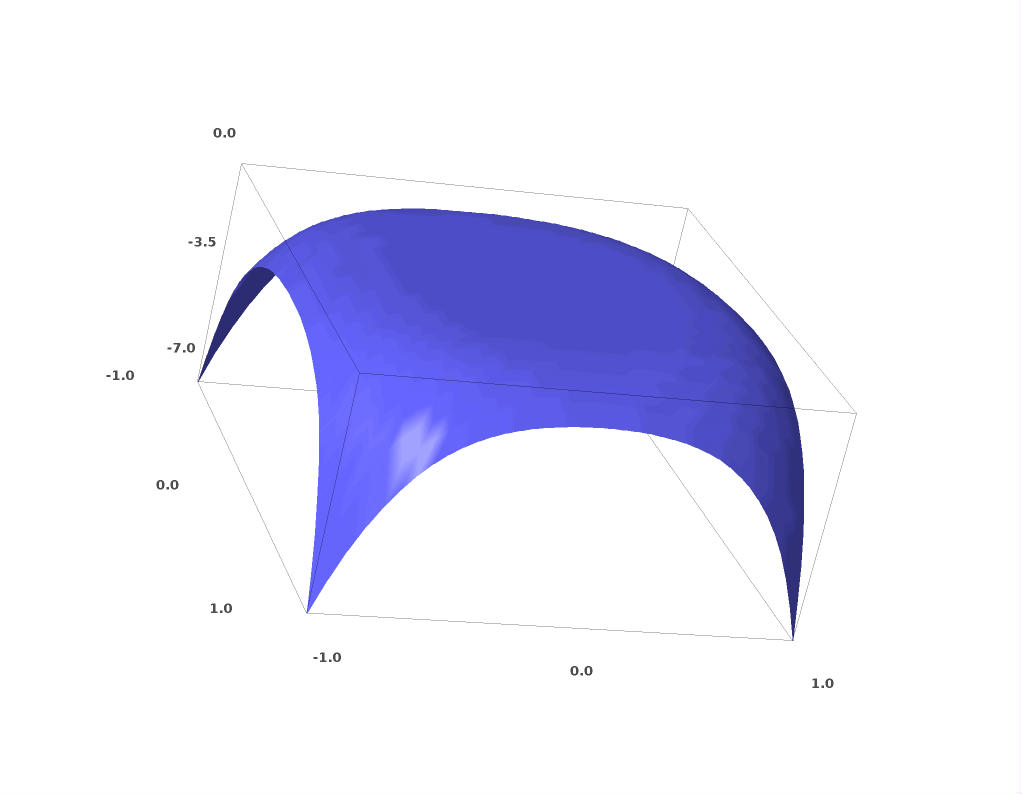
\includegraphics[scale=0.25]{figures/surface_1.jpg}}
\only<2>{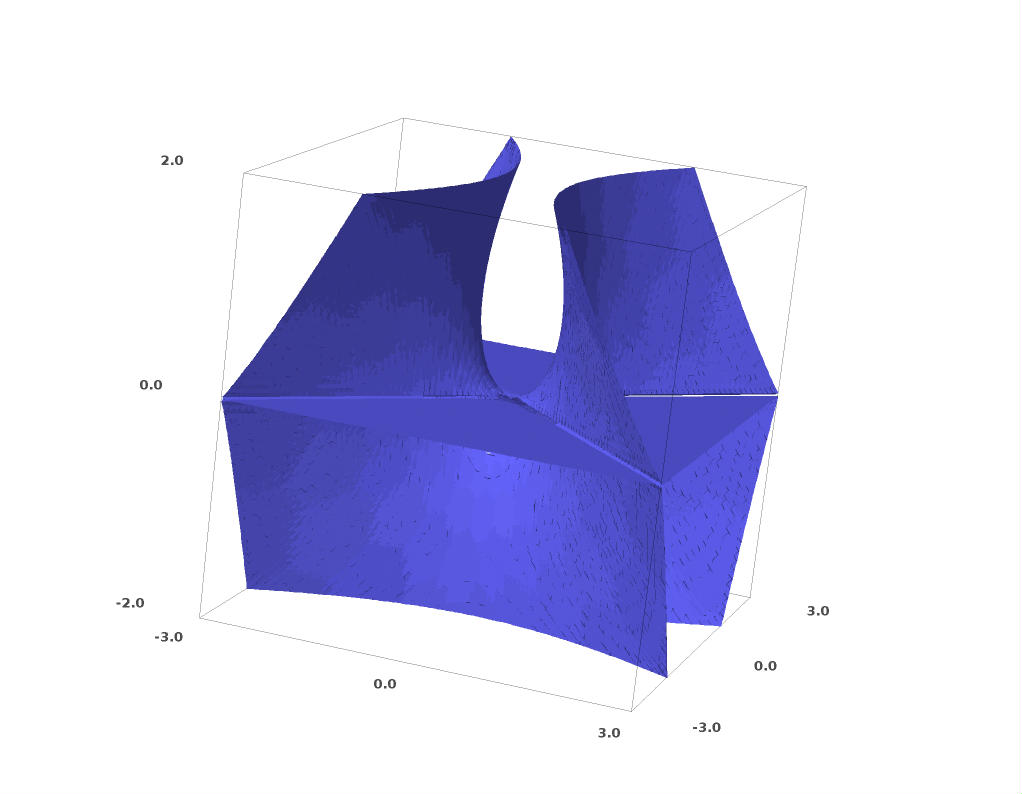
\includegraphics[scale=0.25]{figures/surface_2.jpg}}
\only<3>{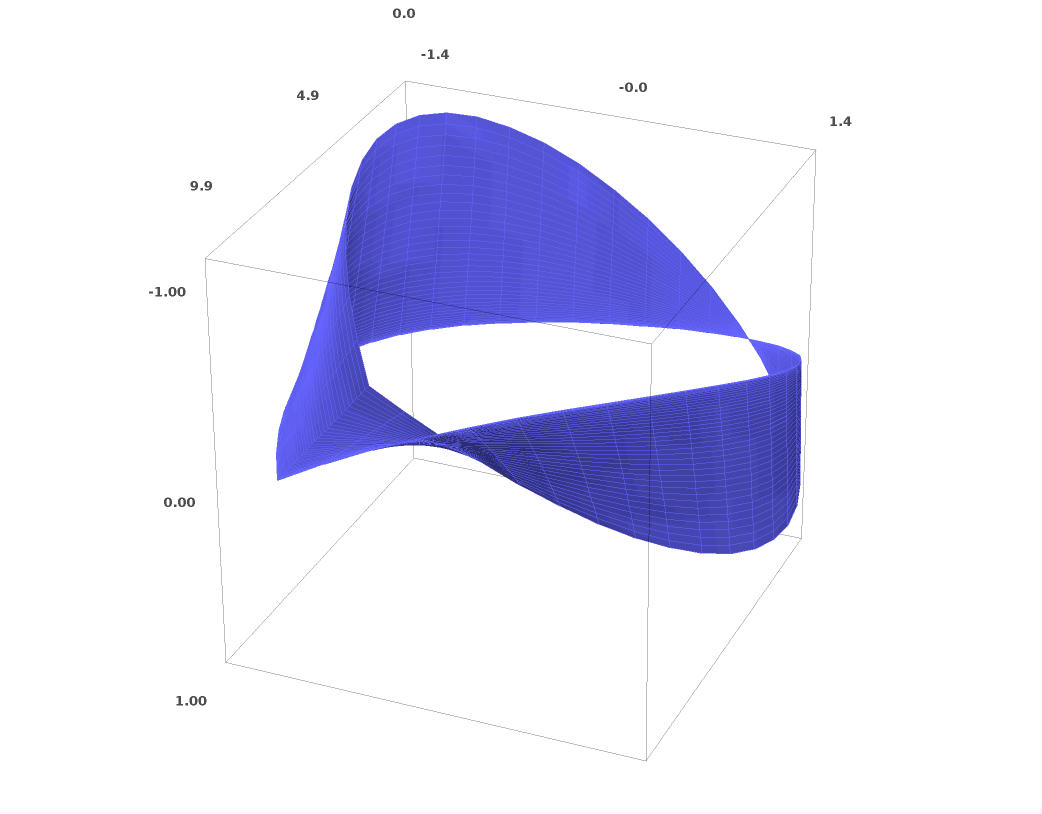
\includegraphics[scale=0.25]{figures/surface_3.jpg}}
\only<4>{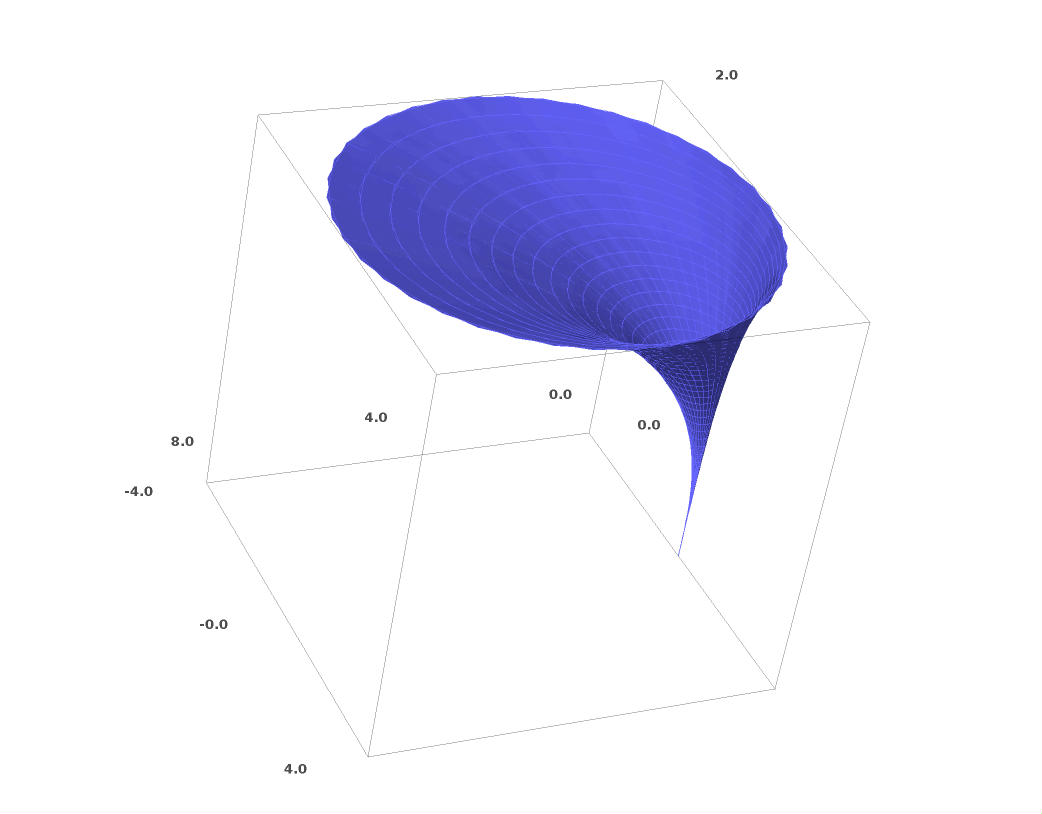
\includegraphics[scale=0.25]{figures/surface_4.jpg}}
\only<5>{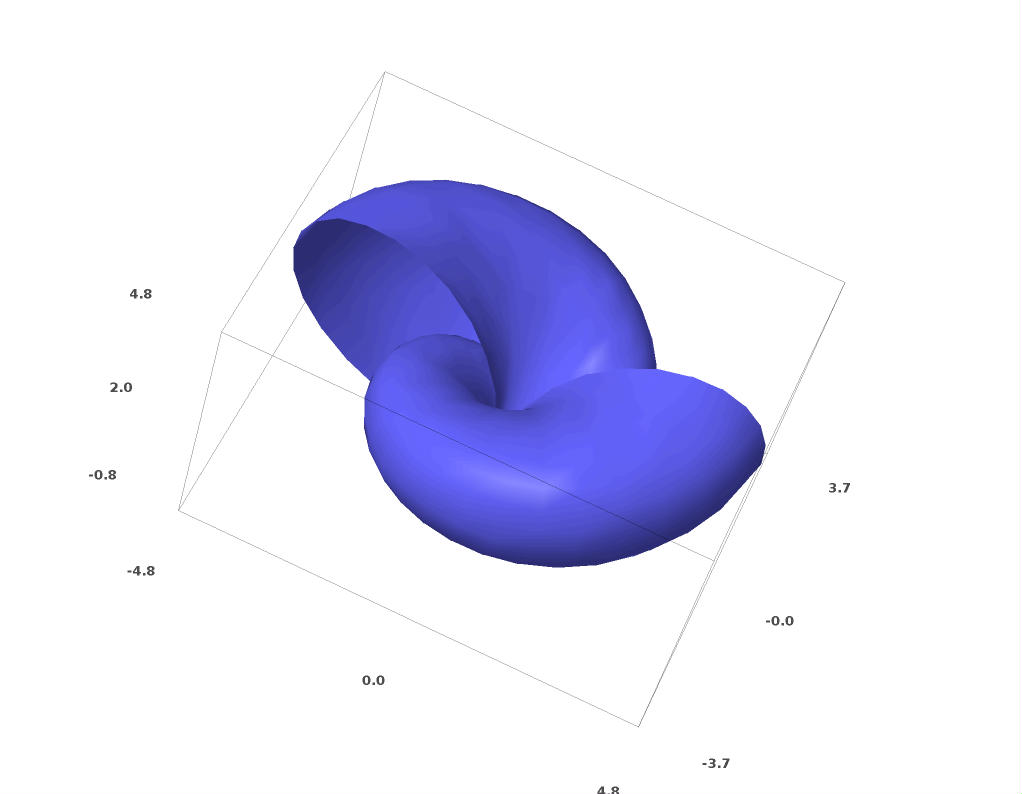
\includegraphics[scale=0.25]{figures/surface_5.jpg}} 
\end{center}
\end{frame}

\end{document}


